\section{Fun with square roots}
\begin{figure}[H]
	\begin{center}
		\begin{tabular}{c c} %% tabular useful for creating an array of images 
			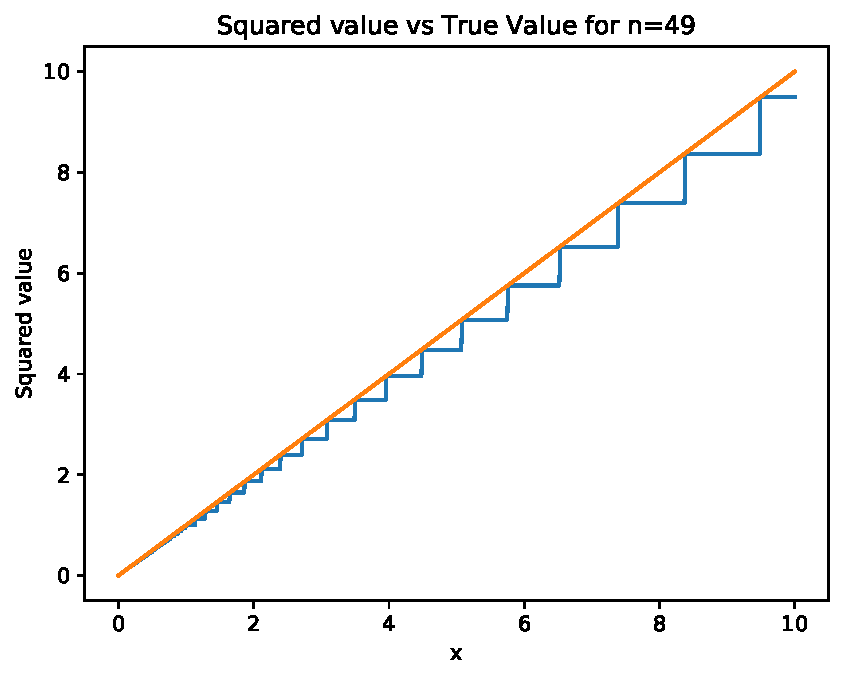
\includegraphics[width=0.45\textwidth]{./figures/plot_for_n_49} & 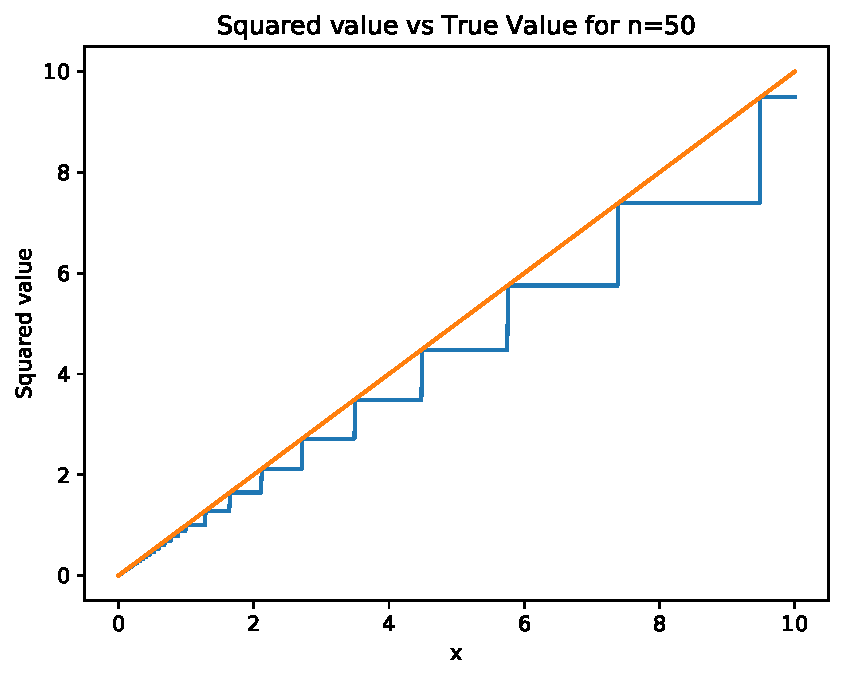
\includegraphics[width=0.45\textwidth]{./figures/plot_for_n_50} \\
			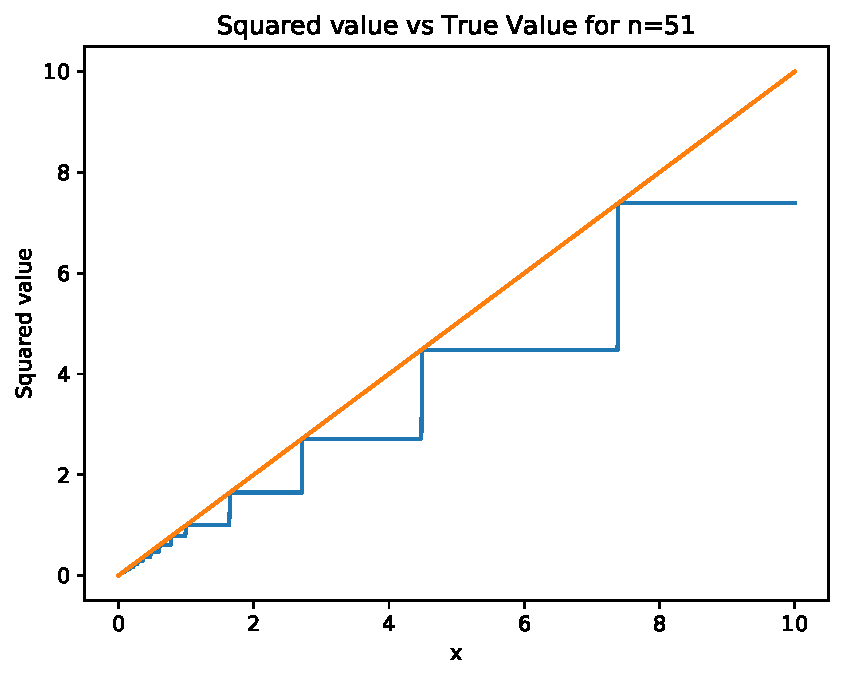
\includegraphics[width=0.45\textwidth]{./figures/plot_for_n_51} & 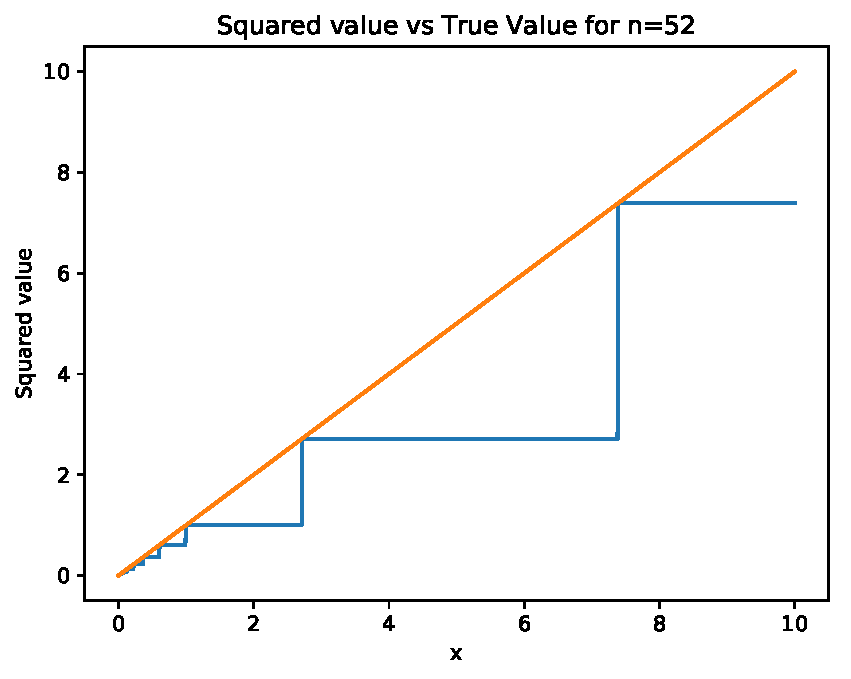
\includegraphics[width=0.45\textwidth]{./figures/plot_for_n_52}
		\end{tabular}
	\end{center}
	\caption[funwithsquareroots] 
	%>>>> use \label inside caption to get Fig. number with \ref{}
	{ Plots for different values of $n$}
\end{figure}